% Build:  cd presentation && tectonic main.tex
% (needs the `ab-initio-pipeline-presentation` conda env — see ../envs/presentation.yaml)
\documentclass[aspectratio=169]{beamer}

\usetheme{default}
\usepackage[utf8]{inputenc}
\usepackage{tikz}
\usetikzlibrary{arrows.meta, positioning, fit}
\usepackage{booktabs}
\usepackage{graphicx}
\graphicspath{{figures/}{figures/logos/}{figures/license/}}

% --- Dark palette: navy / warm-white -------------------------------------
% High-contrast variant of the sibling ABCfold_NPF_pipeline deck's palette,
% picked from a 6-way WCAG-contrast benchmark (presentation/_bench/) because
% the venue's projector washes out mid-tone grays. bg kept close to the
% sibling deck's navy for visual continuity; fg/muted/substrate brightened
% to clear AA/AAA against it (accent kept as-is at 5.79:1, still AA).
%   bg vs fg (body text):    16.95:1 (AAA)
%   bg vs accent (bullets):   5.79:1 (AA)
%   bg vs muted (footline):   7.16:1 (AAA)
%   bg vs substrate (emph):   7.46:1 (AAA)
\definecolor{bgdark}{HTML}{05171F}
\definecolor{fgtext}{HTML}{FDF6E3}
\definecolor{accent}{HTML}{2AA198}   % structure/links/bullets
\definecolor{muted}{HTML}{8FA6AD}    % footline / secondary text
\definecolor{substrate}{HTML}{A29CF2} % this deck's "key takeaway" highlight color

\setbeamertemplate{navigation symbols}{}
\setbeamercolor{background canvas}{bg=bgdark}
\setbeamercolor{normal text}{fg=fgtext, bg=bgdark}
\setbeamercolor{structure}{fg=accent}
\setbeamercolor{title}{fg=fgtext}
\setbeamercolor{subtitle}{fg=muted}
\setbeamercolor{author}{fg=muted}
\setbeamercolor{institute}{fg=muted}
\setbeamercolor{date}{fg=muted}
\setbeamercolor{frametitle}{fg=fgtext, bg=bgdark}
\setbeamercolor{itemize item}{fg=accent}
\setbeamercolor{itemize subitem}{fg=accent}
\setbeamercolor{enumerate item}{fg=accent}
\setbeamertemplate{itemize item}[circle]
\setbeamertemplate{itemize subitem}[circle]
\setbeamercolor{section in toc}{fg=fgtext}
\setbeamercolor{page number in head/foot}{fg=muted}
\setbeamerfont{frametitle}{series=\bfseries}

% --- header: section progress, no per-slide dots -------------------------
\setbeamercolor{section in head/foot}{fg=bgdark, bg=accent}
\setbeamerfont{section in head/foot}{size=\tiny}
\setbeamertemplate{headline}{%
  \begin{beamercolorbox}[wd=\paperwidth, ht=2.5ex, dp=0.9ex]{section in head/foot}
    \usebeamerfont{section in head/foot}\insertsectionnavigationhorizontal{\paperwidth}{}{}
  \end{beamercolorbox}%
}

% --- current subsection name, tracked by hand ----------------------------
\newcommand{\currentsubsectionname}{}
\newcommand{\emptysubsectionname}{}
\let\origsubsection\subsection
\renewcommand{\subsection}[1]{\origsubsection{#1}\gdef\currentsubsectionname{#1}}

\setbeamertemplate{frametitle}{%
  \nointerlineskip
  \begin{beamercolorbox}[wd=\paperwidth, sep=0.3cm]{frametitle}
    \usebeamerfont{frametitle}\insertframetitle\hfill
    \ifx\currentsubsectionname\emptysubsectionname\else
      {\normalfont\footnotesize\color{muted}\currentsubsectionname}%
    \fi
    \strut
  \end{beamercolorbox}%
}
% --- section-divider frame: big centered section name --------------------
\newcommand{\sectiondivider}[1]{%
  {\setbeamertemplate{frametitle}{}%
  \begin{frame}
    \vfill
    \begin{center}
      {\color{accent}\rule{0.35\textwidth}{0.6pt}}\\[1.1em]
      {\color{fgtext}\Huge\bfseries #1}\\[1.1em]
      {\color{accent}\rule{0.35\textwidth}{0.6pt}}
    \end{center}
    \vfill
  \end{frame}}%
}

\setbeamercolor{footlineright}{fg=muted, bg=bgdark}
\setbeamertemplate{footline}{%
  \leavevmode%
  \hbox{%
    \begin{beamercolorbox}[wd=\paperwidth, ht=2.6ex, dp=1.2ex, right, rightskip=0.3cm]{footlineright}
      \usebeamerfont{footline}\tiny CC BY 4.0~\raisebox{-0.15em}{
\includegraphics[height=1.4ex]{by-4.0-88x31.pdf}}\hspace{0.4em}\insertframenumber\,/\,\inserttotalframenumber
    \end{beamercolorbox}%
  }%
}
\makeatletter
\AtBeginDocument{%
  \g@addto@macro{\@listi}{\setlength{\itemsep}{0.5em}\setlength{\topsep}{0.5em}}
  \g@addto@macro{\@listii}{\setlength{\itemsep}{0.5em}\setlength{\topsep}{0.5em}}
}
\makeatother
\setbeamertemplate{sections/subsections in toc}[sections numbered]

\title{A Cookiecutter Template for Ab-initio Complex Modelling}
\subtitle{Generalizing the ABCfold pipeline: architecture, templating, and reporting}
\author{Etienne Reboul}
\institute{Groupe Gibbérellines et adaptation à l'environnement\\
Institut de Biologie Moléculaire des Plantes (IBMP), Strasbourg}
\date{\today}

\begin{document}

{\setbeamercolor{blank head}{bg=bgdark}
\setbeamertemplate{headline}{%
  \begin{beamercolorbox}[wd=\paperwidth, ht=2.5ex, dp=0.9ex]{blank head}\end{beamercolorbox}%
}
\begin{frame}
  \begin{tikzpicture}[remember picture, overlay]
    \node[anchor=north] at ([yshift=-0.5cm]current page.north) {
      
\includegraphics[height=0.8cm]{cnrs-white.png}%
      \hspace{1.4cm}%
      {\setlength{\fboxsep}{4pt}\colorbox{white}{
\includegraphics[height=0.7cm]{ibmp-color.png}}}%
      \hspace{1.4cm}%
      
\includegraphics[height=0.8cm]{anr-white.png}
    };
  \end{tikzpicture}
  \titlepage
\end{frame}

\begin{frame}{Outline}
  \footnotesize
  \begin{columns}[t]
    \begin{column}{0.48\textwidth}
      \tableofcontents[sections={1,2,3}]
    \end{column}
    \begin{column}{0.48\textwidth}
      \tableofcontents[sections={4,5,6,7}]
    \end{column}
  \end{columns}
\end{frame}
}

% ---------------------------------------------------------------------
\section{Introduction}
% ---------------------------------------------------------------------
\gdef\currentsubsectionname{}
\sectiondivider{Introduction}

\begin{frame}{Where this comes from}
  \begin{itemize}
    \item Three one-off pipelines already run the \textbf{same} 3-stage
      protocol (preprocess $\to$ process $\to$ postprocess):
      \begin{itemize}
        \item NPF / ABCfold (gibberellin importers -- this lab's prior talk)
        \item DRB2/DCL4/dsRNA
        \item AGO1/FBW2/miR
      \end{itemize}
    \item Each new dataset meant \textbf{copy the pipeline, hand-edit the
      scripts} -- system names, chain ids, and domain ranges hardcoded
      throughout
    \item[$\Rightarrow$] Same skeleton, three separate codebases to
      maintain and keep in sync
  \end{itemize}
\end{frame}

\begin{frame}{Goals of the generalization}
  \begin{enumerate}
    \item One reusable template: \textbf{generate-and-run}, not
      copy-and-edit
    \item Adding a new dataset = editing \textbf{only} \texttt{config.yaml}'s
      \texttt{systems:} list + one \texttt{configs/<system>.yaml} --
      \textbf{no script edits}
    \item Portable across HPC schedulers: SLURM, PBS, HTCondor
    \item \textbf{Report-first}: every stage ships a self-contained HTML
      report bundle, replacing ad hoc notebook visualization
  \end{enumerate}
\end{frame}

% ---------------------------------------------------------------------
\section{The three-stage pipeline}
% ---------------------------------------------------------------------
\gdef\currentsubsectionname{}
\sectiondivider{The three-stage pipeline}

\begin{frame}{Three stages, one diagram}
  \centering
  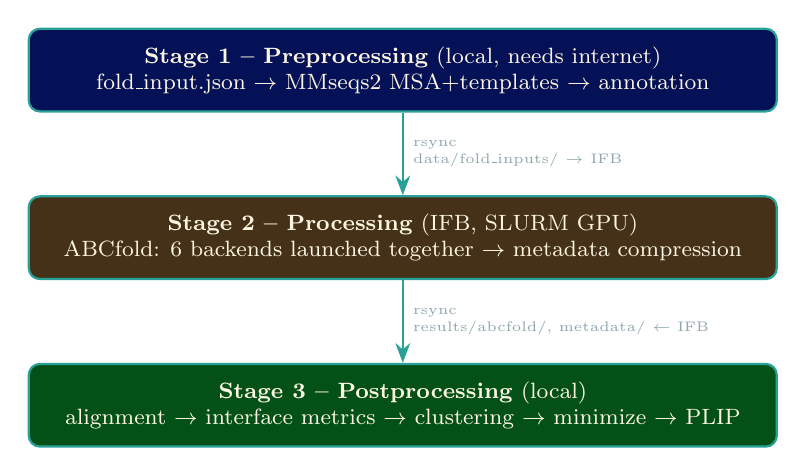
\begin{tikzpicture}[
      every node/.style={text=fgtext},
      stage/.style={draw=accent, thick, rounded corners, minimum width=9.5cm, minimum height=1.05cm,
                     align=center, font=\footnotesize, inner sep=3pt},
      arr/.style={-{Stealth[length=2.5mm]}, thick, draw=accent},
      lbl/.style={font=\tiny, text=muted, align=left}
    ]
    \node[stage, fill=blue!25!bgdark] (pre)  {\textbf{Stage 1 -- Preprocessing} (local, needs internet)\\
                                        fold\_input.json $\to$ MMseqs2 MSA+templates $\to$ annotation};
    \node[stage, fill=orange!25!bgdark, below=1.05cm of pre] (proc) {\textbf{Stage 2 -- Processing} (IFB, SLURM GPU)\\
                                        ABCfold: 6 backends launched together $\to$ metadata compression};
    \node[stage, fill=green!25!bgdark, below=1.05cm of proc] (post) {\textbf{Stage 3 -- Postprocessing} (local)\\
                                        alignment $\to$ interface metrics $\to$ clustering $\to$ minimize $\to$ PLIP};
    \draw[arr] (pre) -- (proc) node[midway, right, lbl] {rsync\\data/fold\_inputs/ $\to$ IFB};
    \draw[arr] (proc) -- (post) node[midway, right, lbl] {rsync\\results/abcfold/, metadata/ $\leftarrow$ IFB};
  \end{tikzpicture}

  \vspace{0.5em}
  {\footnotesize\textcolor{substrate}{\textbf{Each stage ends in a self-contained report bundle}} (\texttt{reports/<stage>.zip}).}\par
\end{frame}

\begin{frame}{Stage 1 -- Preprocessing}
  \begin{itemize}
    \item \textbf{MMseqs2} against the ColabFold webserver: MSA + top-hit
      template search -- offloaded, no local sequence database needed
    \item \textbf{Domain annotation}: ScanProsite + InterProScan REST
    \item \textbf{Disorder prediction}: IUPred3 (long/short) + ANCHOR2 +
      AIUPred
    \item \textbf{MoRF annotation}: MoRFchibi2 (\texttt{tools/MC2})
    \item[$\Rightarrow$] \texttt{fold\_input.json} (holo \& apo forms), with
      a \textbf{human-review gate}: \texttt{annotation\_reviewed: false}
      blocks stage 2 until the curated \texttt{domains:} block is reviewed
  \end{itemize}
\end{frame}

\begin{frame}{Stage 2 -- Processing}
  \begin{itemize}
    \item Snakemake, with a \textbf{pluggable executor plugin} per HPC
      scheduler (SLURM/PBS/HTCondor -- next section)
    \item One SLURM GPU job per system: \textbf{ABCfold} runs all 6
      backends together (\texttt{-abcopr})
    \item Validated on IFB: job \texttt{1840322}, 5 backends $\times$ 3
      seeds = 15 models, $\sim$25~min on an L40S node
    \item Metadata compression: per-model \texttt{ptm}/\texttt{iptm}/
      \texttt{ranking\_score} $\to$ \texttt{arrays.h5} +
      \texttt{model\_metadata.parquet}
  \end{itemize}
\end{frame}

\begin{frame}{The six backends}
  \begin{columns}[T]
    \begin{column}{0.5\textwidth}
      \begin{itemize}
        \setlength{\itemsep}{0.6em}
        \item AlphaFold3\\
          {\fontsize{6pt}{7pt}\selectfont\color{muted}Abramson \textit{et al.}, \textit{Nature} 2024}
        \item Boltz-2\\
          {\fontsize{6pt}{7pt}\selectfont\color{muted}Passaro \textit{et al.}, \textit{bioRxiv} 2025}
        \item Chai-1\\
          {\fontsize{6pt}{7pt}\selectfont\color{muted}Chai Discovery team, \textit{bioRxiv} 2024}
      \end{itemize}
    \end{column}
    \begin{column}{0.5\textwidth}
      \begin{itemize}
        \setlength{\itemsep}{0.6em}
        \item OpenFold3\\
          {\fontsize{6pt}{7pt}\selectfont\color{muted}OpenFold Consortium, technical report, 2025}
        \item Protenix\\
          {\fontsize{6pt}{7pt}\selectfont\color{muted}ByteDance AI4Science, \textit{bioRxiv} 2025}
        \item RosettaFold3\\
          {\fontsize{6pt}{7pt}\selectfont\color{muted}Baker/DiMaio Lab (IPD), Microsoft Foundry, 2025}
      \end{itemize}
    \end{column}
  \end{columns}
  \vspace{0.6em}
  \centering
  All launched via ABCfold, a wrapper that runs multiple backends in one
  call -- pooling backends recovers conformational diversity a single model
  misses (see prior talk).
\end{frame}

\begin{frame}{Stage 3 -- Postprocessing}
  \begin{enumerate}
    \item \textbf{Kabsch alignment} on each rigid anchor
      (\texttt{anchor\_chains}), iteratively refined
    \item \textbf{Interface metrics} over the full ensemble: ipSAE, iLIS,
      Pinc
    \item \textbf{Pose clustering}: HDBSCAN+Optuna/DBCV, or GMM/BIC
    \item Top-N/cluster $\to$ \textbf{ChimeraX minimize} $\to$
      \texttt{fix\_pdb} $\to$ \textbf{PLIP} $\times$ passes $\to$ aggregate
  \end{enumerate}
  \vspace{0.5em}
  \small \texttt{plip\_passes} generalises what used to be several
  hardcoded PLIP configurations (protein--protein, RNA--ligand, mixed)
  into one configurable list per system.
\end{frame}

% ---------------------------------------------------------------------
\section{Turning it into a template}
% ---------------------------------------------------------------------
\gdef\currentsubsectionname{}
\sectiondivider{Turning it into a template}

\begin{frame}{The audit}
  \begin{itemize}
    \item Before templating: does anything in the pipeline or reporting
      logic hardcode a system name, chain id, organism, or account
      \emph{outside} the config layer?
    \item Config layer = \texttt{config.yaml} + \texttt{configs/<system>.yaml}
      + \texttt{config.local.yaml}
    \item Found only a short, enumerable list of non-generic leftovers:
      \begin{itemize}
        \item 2 standalone scripts hardcoding DRB2/DRB4 disorder ranges --
          \textbf{not referenced by any Snakefile}
        \item one \texttt{\_reference/} directory (old submission script,
          kept for reference)
        \item one legacy config-key back-compat shim, dead code
      \end{itemize}
    \item[$\Rightarrow$] \textcolor{substrate}{\textbf{Verdict: go ahead.}}
  \end{itemize}
\end{frame}

\begin{frame}{Template mechanics}
  \footnotesize
  Repo root \textbf{is} the template: \texttt{cookiecutter.json} +
  \texttt{hooks/} at root; every real pipeline file lives under
  \texttt{\{\{cookiecutter.project\_slug\}\}/}.

  \vspace{0.6em}
  \begin{center}
  \begin{tabular}{@{}ll@{}}
    \toprule
    prompt & feeds \\
    \midrule
    \texttt{first\_system\_name} & \texttt{config.yaml systems:} + \texttt{configs/<name>.yaml} \\
    \texttt{project\_slug} & generated directory name \\
    \texttt{contact\_email} & \texttt{config.local.yaml} (InterProScan REST contact) \\
    \texttt{scheduler} & \texttt{config.yaml hpc.scheduler} (slurm/pbs/htcondor) \\
    \texttt{cluster\_account} & \texttt{config.yaml hpc.account} \\
    \texttt{chimerax\_bin} & stage 3 minimization path \\
    \texttt{backends} & subset of the 6 ABCfold backends \\
    \texttt{setup\_first\_system\_now} & triggers interactive FASTA $\to$ config flow \\
    \bottomrule
  \end{tabular}
  \end{center}
\end{frame}

\begin{frame}{Pre/post-gen hooks}
  \begin{itemize}
    \item \textbf{Pre-gen}: validates \texttt{project\_slug}/
      \texttt{first\_system\_name} are filesystem-safe, and that
      \texttt{contact\_email} isn't blank or the placeholder -- EBI's
      InterProScan REST service rejects requests without a real contact
      address
    \item \textbf{Post-gen}:
      \begin{itemize}
        \item drops sibling-only leftovers (the 2 DRB2 scripts,
          \texttt{\_reference/}, empty \texttt{report/captions/})
        \item \textbf{writes \texttt{config.local.yaml}} from
          \texttt{contact\_email} -- this file had always been
          hand-created before; it was the explicit trigger for this whole
          effort
        \item optional: interactive FASTA $\to$
          \texttt{configs/<system>.yaml} flow (chain ids, anchor/partner,
          size class)
        \item \texttt{git init} + initial commit
      \end{itemize}
  \end{itemize}
\end{frame}

\begin{frame}{Adding a new dataset}
  \small Edit \textbf{only}: 1 line in \texttt{config.yaml}'s
  \texttt{systems:} list + 1 new \texttt{configs/<system>.yaml}.
  \textcolor{substrate}{\textbf{No script edits.}}

  \vspace{0.6em}
  {\ttfamily\scriptsize
  \begin{flushleft}
  sequences:\\
  \ -\ \{type: protein, id: A, name: Receptor, sequence: "..."\}\\
  \ -\ \{type: protein, id: B, name: Partner,\ \ sequence: "..."\}\\
  anchor\_chains:\ \ [A]\\
  partner\_chains: [B]\\
  annotation\_reviewed: false\\
  domains:\\
  \ \ A: [\{name: dom1, start: 1, end: 76, kind: domain\}]\\
  plip\_passes:\\
  \ -\ \{name: main, dnareceptor: false, fix\_pdb: false, chains: "[['A'],['B']]"\}\\
  \end{flushleft}
  }
\end{frame}

% ---------------------------------------------------------------------
\section{One config, three schedulers}
% ---------------------------------------------------------------------
\gdef\currentsubsectionname{}
\sectiondivider{One config, three schedulers}

\begin{frame}{Why \texttt{hpc:}, not \texttt{cluster:}}
  \begin{itemize}
    \item Named \texttt{hpc:} to avoid colliding with the pre-existing
      pose-\texttt{cluster:} key used by stage 3
    \item One sub-block per scheduler (\texttt{slurm}/\texttt{pbs}/
      \texttt{htcondor}), each following \textbf{that scheduler's own}
      Snakemake executor plugin's actual documented resource-key
      conventions -- not a made-up common schema
    \item \texttt{run\_abcfold} declares the \textbf{union} of all three
      schedulers' resource keys; a \texttt{res\_*} function gated on
      \texttt{hpc.scheduler} resolves each one
    \item[$\Rightarrow$] inactive schedulers' keys resolve to harmless
      \texttt{0}/\texttt{""} -- no Jinja/conditional templating of the
      Snakefile itself needed
  \end{itemize}
\end{frame}

\begin{frame}{Validated vs.\ untested -- be honest}
  \begin{itemize}
    \item Only \textbf{SLURM} has run a real job -- IFB, job
      \texttt{1840322}
    \item \texttt{pbs}/\texttt{htcondor}: wired from each plugin's own
      README, confirmed to render valid config/resource values for all
      three \texttt{scheduler} choices (\texttt{cookiecutter --no-input} +
      isolated resolver-function tests) -- but \textbf{never run against a
      live pool}
    \item Known gaps if you try one:
      \begin{itemize}
        \item PBS: no native GPU resource; account/queue can't vary by
          \texttt{size\_class}
        \item HTCondor: assumes a shared filesystem between submit/execute
          nodes
      \end{itemize}
  \end{itemize}
\end{frame}

% ---------------------------------------------------------------------
\section{Reports instead of notebooks}
% ---------------------------------------------------------------------
\gdef\currentsubsectionname{}
\sectiondivider{Reports instead of notebooks}

\begin{frame}{Design goals}
  \begin{itemize}
    \item Replace ad hoc notebook visualization with \textbf{Snakemake's
      built-in report}: one self-contained bundle per stage
      (\texttt{reports/<stage>.zip})
    \item \textbf{SVG/PDF figures only}, never raster
    \item \textbf{Dark theme by default} (\texttt{report/custom.css},
      injected via \texttt{--report-stylesheet} -- the underlying report
      app has no native dark mode); \texttt{datavzrd} tables get a
      matching dark skin
    \item[$\Rightarrow$] \textcolor{substrate}{\textbf{Zip, not bare
      \texttt{.html}}}: browsers block the \texttt{data:} URLs a
      single-file report would need to embed interactive tables
  \end{itemize}
\end{frame}

\begin{frame}{Stage 1 \& 2 reports}
  \footnotesize
  \textbf{Stage 1}:
  \begin{itemize}
    \item ColabFold-style MSA coverage/depth plot
    \item Domain bar chart, segmented by domain/linker
    \item Superposed disorder line plots (IUPred3 long/short, ANCHOR2,
      AIUPred)
    \item \texttt{datavzrd} tables: input-file statistics, template-hit
      coverage
  \end{itemize}
  \vspace{0.6em}
  \textbf{Stage 2}:
  \begin{itemize}
    \item \texttt{datavzrd} table: metadata-compression space saved
  \end{itemize}
\end{frame}

\begin{frame}{Stage 3 report}
  \footnotesize
  \begin{itemize}
    \item RMSD violin plots + rigid-core line plot (which residues anchor
      the Kabsch alignment)
    \item Per-backend \texttt{datavzrd} failure-rate table + seaborn
      energy-minimization line plot
    \item Customisable dimensionality-reduction panels
      (PCA/t-SNE/UMAP/MDS), colored by backend, rescoring metric, or
      cluster
    \item PLIP contact heatmaps: per backend / per cluster / total --
      domain-aware for protein--protein, nucleic-acid-aware for
      protein--NA/ligand interfaces
  \end{itemize}
\end{frame}

% ---------------------------------------------------------------------
\section{Does it actually work?}
% ---------------------------------------------------------------------
\gdef\currentsubsectionname{}
\sectiondivider{Does it actually work?}

\begin{frame}{End-to-end toy validation}
  \footnotesize
  \texttt{example\_toy} (ubiquitin homodimer) through all 3 stages:

  \vspace{0.4em}
  \begin{center}
  \begin{tabular}{@{}lll@{}}
    \toprule
    stage & where & result \\
    \midrule
    1 -- preprocessing & local & DAG-clean \\
    2 -- processing & IFB SLURM GPU & job \texttt{1840322}, 15 models, $\sim$25~min (L40S) \\
    3 -- postprocessing & local (ChimeraX/Docker) & 53/53 steps clean \\
    \bottomrule
  \end{tabular}
  \end{center}

  \vspace{0.6em}
  Rough edges found \& fixed along the way: a stale \texttt{snakemake}-module
  SLURM executor plugin that hung silently at job submission, and
  resource-key restrictions in plugin $\geq$2.7 -- both are now committed
  fixes, not open issues.
\end{frame}

\begin{frame}{Current status, honestly}
  \begin{itemize}
    \item \textbf{Proven}: the SLURM path, the reporting layer, the
      cookiecutter mechanics themselves (repeated
      \texttt{cookiecutter --no-input} runs, all three scheduler choices)
    \item \textbf{Still open}:
      \begin{itemize}
        \item PBS/HTCondor unproven against a live pool
        \item \texttt{report/} vs.\ \texttt{reports/} naming -- a real
          footgun, never resolved
        \item docstring/\texttt{Usage:} cleanup sweep only partially done
      \end{itemize}
  \end{itemize}
\end{frame}

% ---------------------------------------------------------------------
\section{Next steps}
% ---------------------------------------------------------------------
\gdef\currentsubsectionname{}
\sectiondivider{Next steps}

\begin{frame}{Roadmap}
  \begin{itemize}
    \item Push this repo to GitHub, so
      \texttt{cookiecutter gh:EtienneReboul/ab\_initio\_pipeline} works
      directly
    \item Get PBS or HTCondor access to actually validate those paths
    \item Apply the template to the \textbf{next real dataset} -- the real
      test of ``2 files, no script edits''
    \item Decide the \texttt{report/}/\texttt{reports/} naming question
  \end{itemize}
\end{frame}

\begin{frame}
  \centering
  \Huge Questions?
\end{frame}

\end{document}
